\chapter{線性表}
這類題目考察線性表的操作,例如,數組,單鏈表,雙向鏈表等。
\newline


\section{數組} %%%%%%%%%%%%%%%%%%%%%%%%%%%%%%


\subsection{Remove Duplicates from Sorted Array}
\label{sec:remove-duplicates-from-sorted-array}


\subsubsection{描述}
Given a sorted array, remove the duplicates in place such that each element appear only once and return the new length.

Do not allocate extra space for another array, you must do this in place with constant memory.

For example, Given input array \code{A = [1,1,2]},

Your function should return length = 2, and A is now \code{\[1,2\]}.


\subsubsection{分析}
無


\subsubsection{代碼1}
\begin{Code}
// LeetCode, Remove Duplicates from Sorted Array
// 時間複雜度O(n),空間複雜度O(1)
class Solution {
public:
    int removeDuplicates(vector<int>& nums) {
        if (nums.empty()) return 0;

        int index = 0;
        for (int i = 1; i < nums.size(); i++) {
            if (nums[index] != nums[i])
                nums[++index] = nums[i];
        }
        return index + 1;
    }
};
\end{Code}


\subsubsection{代碼2}
\begin{Code}
// LeetCode, Remove Duplicates from Sorted Array
// 使用STL,時間複雜度O(n),空間複雜度O(1)
class Solution {
public:
    int removeDuplicates(vector<int>& nums) {
        return distance(nums.begin(), unique(nums.begin(), nums.end()));
    }
};
\end{Code}


\subsubsection{代碼3}
\begin{Code}
// LeetCode, Remove Duplicates from Sorted Array
// 使用STL,時間複雜度O(n),空間複雜度O(1)
class Solution {
public:
    int removeDuplicates(vector<int>& nums) {
        return distance(nums.begin(), removeDuplicates(nums.begin(), nums.end(), nums.begin()));
    }

    template<typename InIt, typename OutIt>
    OutIt removeDuplicates(InIt first, InIt last, OutIt output) {
        while (first != last) {
            *output++ = *first;
            first = upper_bound(first, last, *first);
        }

        return output;
    }
};
\end{Code}


\subsubsection{相關題目}

\begindot
\item Remove Duplicates from Sorted Array II,見 \S \ref{sec:remove-duplicates-from-sorted-array-ii}
\myenddot


\subsection{Remove Duplicates from Sorted Array II}
\label{sec:remove-duplicates-from-sorted-array-ii}


\subsubsection{描述}
Follow up for "Remove Duplicates":
What if duplicates are allowed at most twice?

For example,
Given sorted array \code{A = [1,1,1,2,2,3]},

Your function should return length = 5, and A is now \code{\[1,1,2,2,3\]}


\subsubsection{分析}
加一個變量記錄一下元素出現的次數即可。這題因為是已經排序的數組,所以一個變量即可解決。如果是沒有排序的數組,則需要引入一個hashmap來記錄出現次數。


\subsubsection{代碼1}
\begin{Code}
// LeetCode, Remove Duplicates from Sorted Array II
// 時間複雜度O(n),空間複雜度O(1)
// @author hex108 (https://github.com/hex108)
class Solution {
public:
    int removeDuplicates(vector<int>& nums) {
        if (nums.size() <= 2) return nums.size();

        int index = 2;
        for (int i = 2; i < nums.size(); i++){
            if (nums[i] != nums[index - 2])
                nums[index++] = nums[i];
        }

        return index;
    }
};
\end{Code}


\subsubsection{代碼2}
下面是一個更簡潔的版本。上面的代碼略長,不過擴展性好一些,例如將\fn{occur < 2}改為\fn{occur < 3},就變成了允許重複最多3次。
\begin{Code}
// LeetCode, Remove Duplicates from Sorted Array II
// @author 虞航仲 (http://weibo.com/u/1666779725)
// 時間複雜度O(n),空間複雜度O(1)
class Solution {
public:
    int removeDuplicates(vector<int>& nums) {
        const int n = nums.size();
        int index = 0;
        for (int i = 0; i < n; ++i) {
            if (i > 0 && i < n - 1 && nums[i] == nums[i - 1] && nums[i] == nums[i + 1])
                continue;

            nums[index++] = nums[i];
        }
        return index;
    }
};
\end{Code}


\subsubsection{代碼3}
Variable of duplication
\begin{Code}
// LeetCode, Remove Duplicates from Sorted Array II
// @author 
// 時間複雜度O(n),空間複雜度O(1)
class Solution {
public:
    int removeDuplicates(vector<int>& nums, int du) {
        int index = du;
        for (int i = du; i < (int)nums.size(); i++) {
            if (nums[index - du] != nums[i])
                nums[index++] = nums[i];
        }

        return index;
    }
};
\end{Code}
\subsubsection{相關題目}

\begindot
\item Remove Duplicates from Sorted Array,見 \S \ref{sec:remove-duplicates-from-sorted-array}
\myenddot


\subsection{Search in Rotated Sorted Array}
\label{sec:search-in-rotated-sorted-array}


\subsubsection{描述}
Suppose a sorted array is rotated at some pivot unknown to you beforehand.

(i.e., \code{0 1 2 4 5 6 7} might become \code{4 5 6 7 0 1 2}).

You are given a target value to search. If found in the array return its index, otherwise return -1.

You may assume no duplicate exists in the array.


\subsubsection{分析}
二分查找,難度主要在於左右邊界的確定。


\subsubsection{代碼}
\begin{Code}
// LeetCode, Search in Rotated Sorted Array
// 時間複雜度O(log n),空間複雜度O(1)
class Solution {
public:
    int search(const vector<int>& nums, int target) {
        int first = 0, last = nums.size();
        while (first != last) {
            const int mid = first  + (last - first) / 2;
            if (nums[mid] == target)
                return mid;
            if (nums[first] <= nums[mid]) {
                if (nums[first] <= target && target < nums[mid])
                    last = mid;
                else
                    first = mid + 1;
            } else {
                if (nums[mid] < target && target <= nums[last-1])
                    first = mid + 1;
                else
                    last = mid;
            }
        }
        return -1;
    }
};
\end{Code}


\subsubsection{相關題目}

\begindot
\item Search in Rotated Sorted Array II,見 \S \ref{sec:search-in-rotated-sorted-array-ii}
\myenddot


\subsection{Search in Rotated Sorted Array II}
\label{sec:search-in-rotated-sorted-array-ii}


\subsubsection{描述}
Follow up for "Search in Rotated Sorted Array": What if \emph{duplicates} are allowed?

Would this affect the run-time complexity? How and why?

Write a function to determine if a given target is in the array.


\subsubsection{分析}
允許重複元素,則上一題中如果\fn{A[m]>=A[l]},那麼\fn{[l,m]}為遞增序列的假設就不能成立了,比如\code{\[1,3,1,1,1\]}。

如果\fn{A[m]>=A[l]}不能確定遞增,那就把它拆分成兩個條件:
\begindot
\item 若\fn{A[m]>A[l]},則區間\fn{[l,m]}一定遞增
\item 若\fn{A[m]==A[l]} 確定不了,那就\fn{l++},往下看一步即可。
\myenddot

\subsubsection{代碼}
\begin{Code}
// LeetCode, Search in Rotated Sorted Array II
// 時間複雜度O(n),空間複雜度O(1)
class Solution {
public:
    bool search(const vector<int>& nums, int target) {
        int first = 0, last = nums.size();
        while (first != last) {
            const int mid = first  + (last - first) / 2;
            if (nums[mid] == target)
                return true;
            if (nums[first] < nums[mid]) {
                if (nums[first] <= target && target < nums[mid])
                    last = mid;
                else
                    first = mid + 1;
            } else if (nums[first] > nums[mid]) {
                if (nums[mid] < target && target <= nums[last-1])
                    first = mid + 1;
                else
                    last = mid;
            } else
                //skip duplicate one
                first++;
        }
        return false;
    }
};
\end{Code}


\subsubsection{相關題目}

\begindot
\item Search in Rotated Sorted Array,見 \S \ref{sec:search-in-rotated-sorted-array}
\myenddot


\subsection{Median of Two Sorted Arrays}
\label{sec:median-of-two-sorted-arrays}


\subsubsection{描述}
There are two sorted arrays A and B of size m and n respectively. Find the median of the two sorted arrays. The overall run time complexity should be $O(\log (m+n))$.


\subsubsection{分析}
這是一道非常經典的題。這題更通用的形式是,給定兩個已經排序好的數組,找到兩者所有元素中第$k$大的元素。

$O(m+n)$的解法比較直觀,直接merge兩個數組,然後求第$k$大的元素。

不過我們僅僅需要第$k$大的元素,是不需要“排序”這麼昂貴的操作的。可以用一個計數器,記錄當前已經找到第$m$大的元素了。同時我們使用兩個指針\fn{pA}和\fn{pB},分別指向A和B數組的第一個元素,使用類似於merge sort的原理,如果數組A當前元素小,那麼\fn{pA++},同時\fn{m++};如果數組B當前元素小,那麼\fn{pB++},同時\fn{m++}。最終當$m$等於$k$的時候,就得到了我們的答案,$O(k)$時間,$O(1)$空間。但是,當$k$很接近$m+n$的時候,這個方法還是$O(m+n)$的。

有沒有更好的方案呢?我們可以考慮從$k$入手。如果我們每次都能夠刪除一個一定在第$k$大元素之前的元素,那麼我們需要進行$k$次。但是如果每次我們都刪除一半呢?由於A和B都是有序的,我們應該充分利用這裏面的信息,類似於二分查找,也是充分利用了“有序”。

假設A和B的元素個數都大於$k/2$,我們將A的第$k/2$個元素(即\fn{A[k/2-1]})和B的第$k/2$個元素(即\fn{B[k/2-1]})進行比較,有以下三種情況(為了簡化這裏先假設$k$為偶數,所得到的結論對於$k$是奇數也是成立的):
\begindot
\item \fn{A[k/2-1] == B[k/2-1]}
\item \fn{A[k/2-1] > B[k/2-1]}
\item \fn{A[k/2-1] < B[k/2-1]}
\myenddot

如果\fn{A[k/2-1] < B[k/2-1]},意味着\fn{A[0]}到\fn{A[k/2-1]}的肯定在$A \cup B$的top k元素的範圍內,換句話説,\fn{A[k/2-1]}不可能大於$A \cup B$的第$k$大元素。留給讀者證明。

因此,我們可以放心的刪除A數組的這$k/2$個元素。同理,當\fn{A[k/2-1] > B[k/2-1]}時,可以刪除B數組的$k/2$個元素。

當\fn{A[k/2-1] == B[k/2-1]}時,説明找到了第$k$大的元素,直接返回\fn{A[k/2-1]}或\fn{B[k/2-1]}即可。

因此,我們可以寫一個遞歸函數。那麼函數什麼時候應該終止呢?
\begindot
\item 當A或B是空時,直接返回\fn{B[k-1]}或\fn{A[k-1]};
\item 當\fn{k=1}是,返回\fn{min(A[0], B[0])};
\item 當\fn{A[k/2-1] == B[k/2-1]}時,返回\fn{A[k/2-1]}或\fn{B[k/2-1]}
\myenddot


\subsubsection{代碼}
\begin{Code}
// LeetCode, Median of Two Sorted Arrays
// 時間複雜度O(log(m+n)),空間複雜度O(log(m+n))
class Solution {
public:
    double findMedianSortedArrays(const vector<int>& A, const vector<int>& B) {
        const int m = A.size();
        const int n = B.size();
        int total = m + n;
        if (total & 0x1)
            return find_kth(A.begin(), m, B.begin(), n, total / 2 + 1);
        else
            return (find_kth(A.begin(), m, B.begin(), n, total / 2)
                    + find_kth(A.begin(), m, B.begin(), n, total / 2 + 1)) / 2.0;
    }
private:
    static int find_kth(std::vector<int>::const_iterator A, int m, 
            std::vector<int>::const_iterator B, int n, int k) {
        //always assume that m is equal or smaller than n
        if (m > n) return find_kth(B, n, A, m, k);
        if (m == 0) return *(B + k - 1);
        if (k == 1) return min(*A, *B);

        //divide k into two parts
        int ia = min(k / 2, m), ib = k - ia;
        if (*(A + ia - 1) < *(B + ib - 1))
            return find_kth(A + ia, m - ia, B, n, k - ia);
        else if (*(A + ia - 1) > *(B + ib - 1))
            return find_kth(A, m, B + ib, n - ib, k - ib);
        else
            return A[ia - 1];
    }
};
\end{Code}


\subsubsection{相關題目}

\begindot
\item 無
\myenddot


\subsection{Longest Consecutive Sequence} %%%%%%%%%%%%%%%%%%%%%%%%%%%%%%
\label{sec:longest-consecutive-sequence}


\subsubsection{描述}
Given an unsorted array of integers, find the length of the longest consecutive elements sequence.

For example,
Given \code{\[100, 4, 200, 1, 3, 2\]},
The longest consecutive elements sequence is \code{\[1, 2, 3, 4\]}. Return its length: 4.

Your algorithm should run in $O(n)$ complexity.


\subsubsection{分析}
如果允許$O(n \log n)$的複雜度,那麼可以先排序,可是本題要求$O(n)$。

由於序列裏的元素是無序的,又要求$O(n)$,首先要想到用哈希表。

用一個哈希表 \fn{unordered_map<int, bool> used}記錄每個元素是否使用,對每個元素,以該元素為中心,往左右擴張,直到不連續為止,記錄下最長的長度。


\subsubsection{代碼}
\begin{Code}
// Leet Code, Longest Consecutive Sequence
// 時間複雜度O(n),空間複雜度O(n)
class Solution {
public:
    int longestConsecutive(const vector<int> &nums) {
        unordered_map<int, bool> used;

        for (auto i : nums) used[i] = false;

        int longest = 0;

        for (auto i : nums) {
            if (used[i]) continue;

            int length = 1;

            used[i] = true;

            for (int j = i + 1; used.find(j) != used.end(); ++j) {
                used[j] = true;
                ++length;
            }

            for (int j = i - 1; used.find(j) != used.end(); --j) {
                used[j] = true;
                ++length;
            }

            longest = max(longest, length);
        }

        return longest;
    }
};
\end{Code}

\subsubsection{分析2}
第一直覺是個聚類的操作,應該有union,find的操作.連續序列可以用兩端和長度來表示.
本來用兩端就可以表示,但考慮到查詢的需求,將兩端分別暴露出來.用\fn{unordered_map<int, int> map}來
存儲.原始思路來自於\url{http://discuss.leetcode.com/questions/1070/longest-consecutive-sequence}

\subsubsection{代碼}

\begin{Code}
// Leet Code, Longest Consecutive Sequence
// 時間複雜度O(n),空間複雜度O(n)
// Author: @advancedxy
class Solution {
public:
    int longestConsecutive(vector<int> &nums) {
        unordered_map<int, int> map;
        int size = nums.size();
        int l = 1;
        for (int i = 0; i < size; i++) {
            if (map.find(nums[i]) != map.end()) continue;
            map[nums[i]] = 1;
            if (map.find(nums[i] - 1) != map.end()) {
                l = max(l, mergeCluster(map, nums[i] - 1, nums[i]));
            }
            if (map.find(nums[i] + 1) != map.end()) {
                l = max(l, mergeCluster(map, nums[i], nums[i] + 1));
            }
        }
        return size == 0 ? 0 : l;
    }

private:
    int mergeCluster(unordered_map<int, int> &map, int left, int right) {
        int upper = right + map[right] - 1;
        int lower = left - map[left] + 1;
        int length = upper - lower + 1;
        map[upper] = length;
        map[lower] = length;
        return length;
    }
};
\end{Code}

\subsubsection{相關題目}
\begindot
\item 無
\myenddot


\subsection{Two Sum} %%%%%%%%%%%%%%%%%%%%%%%%%%%%%%
\label{sec:Two-sum}


\subsubsection{描述}
Given an array of integers, find two numbers such that they add up to a specific target number.

The function twoSum should return indices of the two numbers such that they add up to the target, where index1 must be less than index2. Please note that your returned answers (both index1 and index2) are not zero-based.

You may assume that each input would have exactly one solution.

Input:  \code{numbers=\{2, 7, 11, 15\}, target=9}

Output: \code{index1=1, index2=2}


\subsubsection{分析}
方法1:暴力,複雜度$O(n^2)$,會超時

方法2:hash。用一個哈希表,存儲每個數對應的下標,複雜度$O(n)$.

方法3:先排序,然後左右夾逼,排序$O(n\log n)$,左右夾逼$O(n)$,最終$O(n\log n)$。但是注意,這題需要返回的是下標,而不是數字本身,因此這個方法行不通。


\subsubsection{代碼}
\begin{Code}
//LeetCode, Two Sum
// 方法2:hash。用一個哈希表,存儲每個數對應的下標
// 時間複雜度O(n),空間複雜度O(n)
class Solution {
public:
    vector<int> twoSum(vector<int> &nums, int target) {
        unordered_map<int, int> mapping;
        vector<int> result;
        for (int i = 0; i < nums.size(); i++) {
            mapping[nums[i]] = i;
        }
        for (int i = 0; i < nums.size(); i++) {
            const int gap = target - nums[i];
            if (mapping.find(gap) != mapping.end() && mapping[gap] > i) {
                result.push_back(i + 1);
                result.push_back(mapping[gap] + 1);
                break;
            }
        }
        return result;
    }
};
\end{Code}


\subsubsection{相關題目}
\begindot
\item 3Sum, 見 \S \ref{sec:3sum}
\item 3Sum Closest, 見 \S \ref{sec:3sum-closest}
\item 4Sum, 見 \S \ref{sec:4sum}
\myenddot


\subsection{3Sum} %%%%%%%%%%%%%%%%%%%%%%%%%%%%%%
\label{sec:3sum}


\subsubsection{描述}
Given an array $S$ of $n$ integers, are there elements $a, b, c$ in $S$ such that $a + b + c = 0$? Find all unique triplets in the array which gives the sum of zero.

Note:
\begindot
\item Elements in a triplet $(a,b,c)$ must be in non-descending order. (ie, $a \leq b \leq c$)
\item The solution set must not contain duplicate triplets.
\myenddot

For example, given array \code{S = \{-1 0 1 2 -1 -4\}}.

A solution set is:
\begin{Code}
(-1, 0, 1)
(-1, -1, 2)
\end{Code}


\subsubsection{分析}
先排序,然後左右夾逼,複雜度 $O(n^2)$。

這個方法可以推廣到$k$-sum,先排序,然後做$k-2$次循環,在最內層循環左右夾逼,時間複雜度是 $O(\max\{n \log n, n^{k-1}\})$。


\subsubsection{代碼}
\begin{Code}
// LeetCode, 3Sum
// 先排序,然後左右夾逼,注意跳過重複的數,時間複雜度O(n^2),空間複雜度O(1)
class Solution {
    public:
    vector<vector<int>> threeSum(vector<int>& nums) {
        vector<vector<int>> result;
        if (nums.size() < 3) return result;
        sort(nums.begin(), nums.end());
        const int target = 0;
		
        auto last = nums.end();
        for (auto i = nums.begin(); i < last-2; ++i) {
            auto j = i+1;
            if (i > nums.begin() && *i == *(i-1)) continue;
            auto k = last-1;
            while (j < k) {
                if (*i + *j + *k < target) {
                    ++j;
                    while(*j == *(j - 1) && j < k) ++j;
                } else if (*i + *j + *k > target) {
                    --k;
                    while(*k == *(k + 1) && j < k) --k;
                } else {
                    result.push_back({ *i, *j, *k });
                    ++j;
                    --k;
                    while(*j == *(j - 1) && *k == *(k + 1) && j < k) ++j;
                }
            }
        }
        return result;
    }
};
\end{Code}


\subsubsection{相關題目}
\begindot
\item Two sum, 見 \S \ref{sec:Two-sum}
\item 3Sum Closest, 見 \S \ref{sec:3sum-closest}
\item 4Sum, 見 \S \ref{sec:4sum}
\myenddot

\subsection{3Sum Closest} %%%%%%%%%%%%%%%%%%%%%%%%%%%%%%
\label{sec:3sum-closest}


\subsubsection{描述}
Given an array $S$ of $n$ integers, find three integers in $S$ such that the sum is closest to a given number, target. Return the sum of the three integers. You may assume that each input would have exactly one solution.

For example, given array \code{S = \{-1 2 1 -4\}}, and \code{target = 1}.

The sum that is closest to the target is 2. (\code{-1 + 2 + 1 = 2}).


\subsubsection{分析}
先排序,然後左右夾逼,複雜度 $O(n^2)$。


\subsubsection{代碼}
\begin{Code}
// LeetCode, 3Sum Closest
// 先排序,然後左右夾逼,時間複雜度O(n^2),空間複雜度O(1)
class Solution {
public:
    int threeSumClosest(vector<int>& nums, int target) {
        int result = 0;
        int min_gap = INT_MAX;

        sort(nums.begin(), nums.end());

        for (auto a = nums.begin(); a != prev(nums.end(), 2); ++a) {
            auto b = next(a);
            auto c = prev(nums.end());

            while (b < c) {
                const int sum = *a + *b + *c;
                const int gap = abs(sum - target);

                if (gap < min_gap) {
                    result = sum;
                    min_gap = gap;
                }

                if (sum < target) ++b;
                else              --c;
            }
        }

        return result;
    }
};
\end{Code}


\subsubsection{相關題目}
\begindot
\item Two sum, 見 \S \ref{sec:Two-sum}
\item 3Sum, 見 \S \ref{sec:3sum}
\item 4Sum, 見 \S \ref{sec:4sum}
\myenddot


\subsection{4Sum} %%%%%%%%%%%%%%%%%%%%%%%%%%%%%%
\label{sec:4sum}


\subsubsection{描述}
Given an array $S$ of $n$ integers, are there elements $a, b, c$, and $d$ in $S$ such that $a + b + c + d = target$? Find all unique quadruplets in the array which gives the sum of target.

Note:
\begindot
\item Elements in a quadruplet $(a,b,c,d)$ must be in non-descending order. (ie, $a \leq b \leq c \leq d$)
\item The solution set must not contain duplicate quadruplets.
\myenddot

For example, given array \code{S = \{1 0 -1 0 -2 2\}}, and \code{target = 0}. 

A solution set is:
\begin{Code}
(-1,  0, 0, 1)
(-2, -1, 1, 2)
(-2,  0, 0, 2)
\end{Code}


\subsubsection{分析}
先排序,然後左右夾逼,複雜度 $O(n^3)$,會超時。

可以用一個hashmap先緩存兩個數的和,最終複雜度$O(n^3)$。這個策略也適用於 3Sum 。


\subsubsection{左右夾逼}
\begin{Code}
// LeetCode, 4Sum
// 先排序,然後左右夾逼,時間複雜度O(n^3),空間複雜度O(1)
class Solution {
public:
    vector<vector<int>> fourSum(vector<int>& nums, int target) {
        vector<vector<int>> result;
        if (nums.size() < 4) return result;
        sort(nums.begin(), nums.end());

        auto last = nums.end();
        for (auto a = nums.begin(); a < prev(last, 3); ++a) {
            for (auto b = next(a); b < prev(last, 2); ++b) {
                auto c = next(b);
                auto d = prev(last);
                while (c < d) {
                    if (*a + *b + *c + *d < target) {
                        ++c;
                    } else if (*a + *b + *c + *d > target) {
                        --d;
                    } else {
                        result.push_back({ *a, *b, *c, *d });
                        ++c;
                        --d;
                    }
                }
            }
        }
        sort(result.begin(), result.end());
        result.erase(unique(result.begin(), result.end()), result.end());
        return result;
    }
};
\end{Code}


\subsubsection{map做緩存}
\begin{Code}
// LeetCode, 4Sum
// 用一個hashmap先緩存兩個數的和
// 時間複雜度,平均O(n^2),最壞O(n^4),空間複雜度O(n^2)
class Solution {
public:
    vector<vector<int> > fourSum(vector<int> &nums, int target) {
        vector<vector<int>> result;
        if (nums.size() < 4) return result;
        sort(nums.begin(), nums.end());

        unordered_map<int, vector<pair<int, int> > > cache;
        for (size_t a = 0; a < nums.size(); ++a) {
            for (size_t b = a + 1; b < nums.size(); ++b) {
                cache[nums[a] + nums[b]].push_back(pair<int, int>(a, b));
            }
        }

        for (int c = 0; c < nums.size(); ++c) {
            for (size_t d = c + 1; d < nums.size(); ++d) {
                const int key = target - nums[c] - nums[d];
                if (cache.find(key) == cache.end()) continue;

                const auto& vec = cache[key];
                for (size_t k = 0; k < vec.size(); ++k) {
                    if (c <= vec[k].second)
                        continue; // 有重疊

                    result.push_back( { nums[vec[k].first],
                            nums[vec[k].second], nums[c], nums[d] });
                }
            }
        }
        sort(result.begin(), result.end());
        result.erase(unique(result.begin(), result.end()), result.end());
        return result;
    }
};
\end{Code}


\subsubsection{multimap}
\begin{Code}
// LeetCode, 4Sum
// 用一個 hashmap 先緩存兩個數的和
// 時間複雜度O(n^2),空間複雜度O(n^2)
// @author 龔陸安(http://weibo.com/luangong)
class Solution {
public:
    vector<vector<int>> fourSum(vector<int>& nums, int target) {
        vector<vector<int>> result;
        if (nums.size() < 4) return result;
        sort(nums.begin(), nums.end());

        unordered_multimap<int, pair<int, int>> cache;
        for (int i = 0; i + 1 < nums.size(); ++i)
            for (int j = i + 1; j < nums.size(); ++j)
                cache.insert(make_pair(nums[i] + nums[j], make_pair(i, j)));

        for (auto i = cache.begin(); i != cache.end(); ++i) {
            int x = target - i->first;
            auto range = cache.equal_range(x);
            for (auto j = range.first; j != range.second; ++j) {
                auto a = i->second.first;
                auto b = i->second.second;
                auto c = j->second.first;
                auto d = j->second.second;
                if (a != c && a != d && b != c && b != d) {
                    vector<int> vec = { nums[a], nums[b], nums[c], nums[d] };
                    sort(vec.begin(), vec.end());
                    result.push_back(vec);
                }
            }
        }
        sort(result.begin(), result.end());
        result.erase(unique(result.begin(), result.end()), result.end());
        return result;
    }
};
\end{Code}


\subsubsection{方法4}
\begin{Code}
// LeetCode, 4Sum
// 先排序,然後左右夾逼,時間複雜度O(n^3logn),空間複雜度O(1),會超時
// 跟方法1相比,表面上優化了,實際上更慢了,切記!
class Solution {
public:
    vector<vector<int>> fourSum(vector<int>& nums, int target) {
        vector<vector<int>> result;
        if (nums.size() < 4) return result;
        sort(nums.begin(), nums.end());

        auto last = nums.end();
        for (auto a = nums.begin(); a < prev(last, 3);
                a = upper_bound(a, prev(last, 3), *a)) {
            for (auto b = next(a); b < prev(last, 2);
                    b = upper_bound(b, prev(last, 2), *b)) {
                auto c = next(b);
                auto d = prev(last);
                while (c < d) {
                    if (*a + *b + *c + *d < target) {
                        c = upper_bound(c, d, *c);
                    } else if (*a + *b + *c + *d > target) {
                        d = prev(lower_bound(c, d, *d));
                    } else {
                        result.push_back({ *a, *b, *c, *d });
                        c = upper_bound(c, d, *c);
                        d = prev(lower_bound(c, d, *d));
                    }
                }
            }
        }
        return result;
    }
};
\end{Code}


\subsubsection{相關題目}
\begindot
\item Two sum, 見 \S \ref{sec:Two-sum}
\item 3Sum, 見 \S \ref{sec:3sum}
\item 3Sum Closest, 見 \S \ref{sec:3sum-closest}
\myenddot


\subsection{Remove Element} %%%%%%%%%%%%%%%%%%%%%%%%%%%%%%
\label{sec:remove-element }


\subsubsection{描述}
Given an array and a value, remove all instances of that value in place and return the new length.

The order of elements can be changed. It doesn't matter what you leave beyond the new length.


\subsubsection{分析}
無


\subsubsection{代碼1}
\begin{Code}
// LeetCode, Remove Element
// 時間複雜度O(n),空間複雜度O(1)
class Solution {
public:
    int removeElement(vector<int>& nums, int target) {
        int index = 0;
        for (int i = 0; i < nums.size(); ++i) {
            if (nums[i] != target) {
                nums[index++] = nums[i];
            }
        }
        return index;
    }
};
\end{Code}


\subsubsection{代碼2}
\begin{Code}
// LeetCode, Remove Element
// 使用remove(),時間複雜度O(n),空間複雜度O(1)
class Solution {
public:
    int removeElement(vector<int>& nums, int target) {
        return distance(nums.begin(), remove(nums.begin(), nums.end(), target));
    }
};
\end{Code}


\subsubsection{相關題目}
\begindot
\item 無
\myenddot


\subsection{Next Permutation} %%%%%%%%%%%%%%%%%%%%%%%%%%%%%%
\label{sec:next-permutation}


\subsubsection{描述}
Implement next permutation, which rearranges numbers into the lexicographically next greater permutation of numbers.

If such arrangement is not possible, it must rearrange it as the lowest possible order (ie, sorted in ascending order).

The replacement must be in-place, do not allocate extra memory.

Here are some examples. Inputs are in the left-hand column and its corresponding outputs are in the right-hand column.
\begin{Code}
1,2,3 → 1,3,2
3,2,1 → 1,2,3
1,1,5 → 1,5,1
\end{Code}


\subsubsection{分析}
算法過程如圖~\ref{fig:permutation}所示(來自\myurl{http://fisherlei.blogspot.com/2012/12/leetcode-next-permutation.html})。

\begin{center}
\includegraphics[width=360pt]{next-permutation.png}\\
\figcaption{下一個排列算法流程}\label{fig:permutation}
\end{center}


\subsubsection{代碼}
\begin{Code}
// LeetCode, Next Permutation
// 時間複雜度O(n),空間複雜度O(1)
class Solution {
public:
    void nextPermutation(vector<int> &nums) {
        next_permutation(nums.begin(), nums.end());
    }

    template<typename BidiIt>
    bool next_permutation(BidiIt first, BidiIt last) {
        // Get a reversed range to simplify reversed traversal.
        const auto rfirst = reverse_iterator<BidiIt>(last);
        const auto rlast = reverse_iterator<BidiIt>(first);

        // Begin from the second last element to the first element.
        auto pivot = next(rfirst);

        // Find `pivot`, which is the first element that is no less than its
        // successor.  `Prev` is used since `pivort` is a `reversed_iterator`.
        while (pivot != rlast && *pivot >= *prev(pivot))
            ++pivot;

        // No such elemenet found, current sequence is already the largest
        // permutation, then rearrange to the first permutation and return false.
        if (pivot == rlast) {
            reverse(rfirst, rlast);
            return false;
        }

        // Scan from right to left, find the first element that is greater than
        // `pivot`.
        auto change = find_if(rfirst, pivot, bind1st(less<int>(), *pivot));

        swap(*change, *pivot);
        reverse(rfirst, pivot);

        return true;
    }
};
\end{Code}


\subsubsection{相關題目}
\begindot
\item Permutation Sequence, 見 \S \ref{sec:permutation-sequence}
\item Permutations, 見 \S \ref{sec:permutations}
\item Permutations II, 見 \S \ref{sec:permutations-ii}
\item Combinations, 見 \S \ref{sec:combinations}
\myenddot

\subsection{Prev Permutation} %%%%%%%%%%%%%%%%%%%%%%%%%%%%%%
\label{sec:prev-permutation}


\subsubsection{描述}
Implement previous permutation

\begin{Code}
1,2,3 → 3,2,1
3,2,1 → 3,1,2
1,1,5 → 5,1,1
\end{Code}


\subsubsection{分析}
無

\subsubsection{代碼}
\begin{Code}
// LeetCode, Previous Permutation
// 時間複雜度O(n),空間複雜度O(1)
class Solution {
public:
    void prevPermutation(vector<int> &nums) {
        prev_permutation(nums.begin(), nums.end());
    }

    template<typename BidiIt>
    bool prev_permutation(BidiIt first, BidiIt last) {
        const auto rfirst = reverse_iterator<BidiIt>(last);
        const auto rlast = reverse_iterator<BidiIt>(first);

        auto pivot = next(rfirst);

        while (pivot != rlast && *(pivot) <= *prev(pivot))
            pivot++;

        if (pivot == rlast) {
            reverse(rfirst, rlast);
            return false;
        }

        auto change = find_if(rfirst, pivot, bind1st(greater<int>(), *pivot));

        swap(*change, *pivot);
        reverse(rfirst, pivot);

        return true;
    }
};
\end{Code}


\subsubsection{相關題目}
\begindot
\item Permutation Sequence, 見 \S \ref{sec:permutation-sequence}
\item Permutations, 見 \S \ref{sec:permutations}
\item Permutations II, 見 \S \ref{sec:permutations-ii}
\item Combinations, 見 \S \ref{sec:combinations}
\myenddot

\subsection{Permutation Sequence} %%%%%%%%%%%%%%%%%%%%%%%%%%%%%%
\label{sec:permutation-sequence}


\subsubsection{描述}
The set \fn{[1,2,3,…,n]} contains a total of $n!$ unique permutations.

By listing and labeling all of the permutations in order,
We get the following sequence (ie, for $n = 3$):
\begin{Code}
"123"
"132"
"213"
"231"
"312"
"321"
\end{Code}

Given $n$ and $k$, return the kth permutation sequence.

Note: Given $n$ will be between 1 and 9 inclusive.


\subsubsection{分析}
簡單的,可以用暴力枚舉法,調用 $k-1$ 次 \fn{next_permutation()}。

暴力枚舉法把前 $k$個排列都求出來了,比較浪費,而我們只需要第$k$個排列。

利用康託編碼的思路,假設有$n$個不重複的元素,第$k$個排列是$a_1, a_2, a_3, ..., a_n$,那麼$a_1$是哪一個位置呢?

我們把$a_1$去掉,那麼剩下的排列為
$a_2, a_3, ..., a_n$, 共計$n-1$個元素,$n-1$個元素共有$(n-1)!$個排列,於是就可以知道 $a_1 = k / (n-1)!$。

同理,$a_2, a_3, ..., a_n$的值推導如下:

\begin{eqnarray}
k_2 &=& k\%(n-1)! \nonumber \\
a_2 &=& k_2/(n-2)! \nonumber \\
\quad & \cdots \nonumber \\
k_{n-1} &=& k_{n-2}\%2! \nonumber \\
a_{n-1} &=& k_{n-1}/1! \nonumber \\
a_n &=& 0 \nonumber
\end{eqnarray}


\subsubsection{使用next_permutation()}
\begin{Code}
// LeetCode, Permutation Sequence
// 使用next_permutation(),TLE
class Solution {
public:
    string getPermutation(int n, int k) {
        string s(n, '0');
        for (int i = 0; i < n; ++i)
            s[i] += i+1;
        for (int i = 0; i < k-1; ++i)
            next_permutation(s.begin(), s.end());
        return s;
    }

    template<typename BidiIt>
    bool next_permutation(BidiIt first, BidiIt last) {
        // 代碼見上一題 Next Permutation
    }
};
\end{Code}


\subsubsection{康託編碼}
\begin{Code}
// LeetCode, Permutation Sequence
// 康託編碼,時間複雜度O(n),空間複雜度O(1)
class Solution {
public:
    string getPermutation(int n, int k) {
        string s(n, '0');
        string result;
        for (int i = 0; i < n; ++i)
            s[i] += i + 1;

        return kth_permutation(s, k);
    }
private:
    int factorial(int n) {
        int result = 1;
        for (int i = 1; i <= n; ++i)
            result *= i;
        return result;
    }

    // seq 已排好序,是第一個排列
    template<typename Sequence>
    Sequence kth_permutation(const Sequence &seq, int k) {
        const int n = seq.size();
        Sequence S(seq);
        Sequence result;

        int base = factorial(n - 1);
        --k;  // 康託編碼從0開始

        for (int i = n - 1; i > 0; k %= base, base /= i, --i) {
            auto a = next(S.begin(), k / base);
            result.push_back(*a);
            S.erase(a);
        }

        result.push_back(S[0]); // 最後一個
        return result;
    }
};
\end{Code}


\subsubsection{相關題目}
\begindot
\item Next Permutation, 見 \S \ref{sec:next-permutation}
\item Permutations, 見 \S \ref{sec:permutations}
\item Permutations II, 見 \S \ref{sec:permutations-ii}
\item Combinations, 見 \S \ref{sec:combinations}
\myenddot


\subsection{Valid Sudoku} %%%%%%%%%%%%%%%%%%%%%%%%%%%%%%
\label{sec:valid-sudoku}


\subsubsection{描述}
Determine if a Sudoku is valid, according to: Sudoku Puzzles - The Rules \myurl{http://sudoku.com.au/TheRules.aspx} .

The Sudoku board could be partially filled, where empty cells are filled with the character \fn{'.'}.

\begin{center}
\includegraphics[width=150pt]{sudoku.png}\\
\figcaption{A partially filled sudoku which is valid}\label{fig:sudoku}
\end{center}

\subsubsection{分析}
細節實現題。


\subsubsection{代碼}
\begin{Code}
// LeetCode, Valid Sudoku
// 時間複雜度O(n^2),空間複雜度O(1)
class Solution {
public:
    bool isValidSudoku(const vector<vector<char>>& board) {
        bool used[9];

        for (int i = 0; i < 9; ++i) {
            fill(used, used + 9, false);

            for (int j = 0; j < 9; ++j) // 檢查行
                if (!check(board[i][j], used))
                    return false;

            fill(used, used + 9, false);

            for (int j = 0; j < 9; ++j) // 檢查列
                if (!check(board[j][i], used))
                    return false;
        }

        for (int r = 0; r < 3; ++r) // 檢查 9 個子格子
            for (int c = 0; c < 3; ++c) {
                fill(used, used + 9, false);

                for (int i = r * 3; i < r * 3 + 3; ++i)
                    for (int j = c * 3; j < c * 3 + 3; ++j)
                        if (!check(board[i][j], used))
                            return false;
            }

        return true;
    }

    bool check(char ch, bool used[9]) {
        if (ch == '.') return true;

        if (used[ch - '1']) return false;

        return used[ch - '1'] = true;
    }
};
\end{Code}


\subsubsection{相關題目}
\begindot
\item Sudoku Solver, 見 \S \ref{sec:sudoku-solver}
\myenddot


\subsection{Trapping Rain Water} %%%%%%%%%%%%%%%%%%%%%%%%%%%%%%
\label{sec:trapping-rain-water}


\subsubsection{描述}
Given $n$ non-negative integers representing an elevation map where the width of each bar is 1, compute how much water it is able to trap after raining.

For example, 
Given \code{\[0,1,0,2,1,0,1,3,2,1,2,1\]}, return 6.

\begin{center}
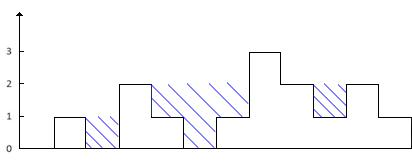
\includegraphics{trapping-rain-water.png}\\
\figcaption{Trapping Rain Water}\label{fig:trapping-rain-water}
\end{center}


\subsubsection{分析}
對於每個柱子,找到其左右兩邊最高的柱子,該柱子能容納的面積就是\code{min(max_left, max_right) - height}。所以,
\begin{enumerate}
\item 從左往右掃描一遍,對於每個柱子,求取左邊最大值;
\item 從右往左掃描一遍,對於每個柱子,求最大右值;
\item 再掃描一遍,把每個柱子的面積並累加。
\end{enumerate}

也可以,
\begin{enumerate}
\item 掃描一遍,找到最高的柱子,這個柱子將數組分為兩半;
\item 處理左邊一半;
\item 處理右邊一半。
\end{enumerate}


\subsubsection{代碼1}
\begin{Code}
// LeetCode, Trapping Rain Water
// 思路1,時間複雜度O(n),空間複雜度O(n)
class Solution {
public:
    int trap(const vector<int>& A) {
        const int n = A.size();
        int *max_left = new int[n]();
        int *max_right = new int[n]();

        for (int i = 1; i < n; i++) {
            max_left[i] = max(max_left[i - 1], A[i - 1]);
            max_right[n - 1 - i] = max(max_right[n - i], A[n - i]);

        }

        int sum = 0;
        for (int i = 0; i < n; i++) {
            int height = min(max_left[i], max_right[i]);
            if (height > A[i]) {
                sum += height - A[i];
            }
        }

        delete[] max_left;
        delete[] max_right;
        return sum;
    }
};
\end{Code}


\subsubsection{代碼2}
\begin{Code}
// LeetCode, Trapping Rain Water
// 思路2,時間複雜度O(n),空間複雜度O(1)
class Solution {
public:
    int trap(const vector<int>& A) {
        const int n = A.size();
        int max = 0; // 最高的柱子,將數組分為兩半
        for (int i = 0; i < n; i++)
            if (A[i] > A[max]) max = i;

        int water = 0;
        for (int i = 0, peak = 0; i < max; i++)
            if (A[i] > peak) peak = A[i];
            else water += peak - A[i];
        for (int i = n - 1, top = 0; i > max; i--)
            if (A[i] > top) top = A[i];
            else water += top - A[i];
        return water;
    }
};
\end{Code}


\subsubsection{代碼3}
第三種解法,用一個棧輔助,小於棧頂的元素壓入,大於等於棧頂就把棧裏所有小於或等於當前值的元素全部出棧處理掉。
\begin{Code}
// LeetCode, Trapping Rain Water
// 用一個棧輔助,小於棧頂的元素壓入,大於等於棧頂就把棧裏所有小於或
// 等於當前值的元素全部出棧處理掉,計算面積,最後把當前元素入棧
// 時間複雜度O(n),空間複雜度O(n)
class Solution {
public:
    int trap(const vector<int>& A) {
        const int n = A.size();
        stack<pair<int, int>> s;
        int water = 0;

        for (int i = 0; i < n; ++i) {
            int height = 0;

            while (!s.empty()) { // 將棧裏比當前元素矮或等高的元素全部處理掉
                int bar = s.top().first;
                int pos = s.top().second;
                // bar, height, A[i] 三者夾成的凹陷
                water += (min(bar, A[i]) - height) * (i - pos - 1);
                height = bar;

                if (A[i] < bar) // 碰到了比當前元素高的,跳出循環
                    break;
                else
                    s.pop(); // 彈出棧頂,因為該元素處理完了,不再需要了
            }

            s.push(make_pair(A[i], i));
        }

        return water;
    }
};
\end{Code}


\subsubsection{相關題目}
\begindot
\item Container With Most Water, 見 \S \ref{sec:container-with-most-water}
\item Largest Rectangle in Histogram, 見 \S \ref{sec:largest-rectangle-in-histogram}
\myenddot


\subsection{Rotate Image} %%%%%%%%%%%%%%%%%%%%%%%%%%%%%%
\label{sec:rotate-image}


\subsubsection{描述}
You are given an $n \times n$ 2D matrix representing an image.

Rotate the image by 90 degrees (clockwise).

Follow up:
Could you do this in-place?


\subsubsection{分析}
首先想到,純模擬,從外到內一圈一圈的轉,但這個方法太慢。

如下圖,首先沿着副對角線翻轉一次,然後沿着水平中線翻轉一次。

\begin{center}
\includegraphics[width=200pt]{rotate-image.png}\\
\figcaption{Rotate Image}\label{fig:rotate-image}
\end{center}

或者,首先沿着水平中線翻轉一次,然後沿着主對角線翻轉一次。


\subsubsection{代碼1}
\begin{Code}
// LeetCode, Rotate Image
// 思路 1,時間複雜度O(n^2),空間複雜度O(1)
class Solution {
public:
    void rotate(vector<vector<int>>& matrix) {
        const int n = matrix.size();

        for (int i = 0; i < n; ++i)  // 沿着副對角線反轉
            for (int j = 0; j < n - i; ++j)
                swap(matrix[i][j], matrix[n - 1 - j][n - 1 - i]);

        for (int i = 0; i < n / 2; ++i) // 沿着水平中線反轉
            for (int j = 0; j < n; ++j)
                swap(matrix[i][j], matrix[n - 1 - i][j]);
    }
};
\end{Code}

\subsubsection{代碼2}
\begin{Code}
// LeetCode, Rotate Image
// 思路 2,時間複雜度O(n^2),空間複雜度O(1)
class Solution {
public:
    void rotate(vector<vector<int>>& matrix) {
        const int n = matrix.size();

        for (int i = 0; i < n / 2; ++i) // 沿着水平中線反轉
            for (int j = 0; j < n; ++j)
                swap(matrix[i][j], matrix[n - 1 - i][j]);

        for (int i = 0; i < n; ++i)  // 沿着主對角線反轉
            for (int j = i + 1; j < n; ++j)
                swap(matrix[i][j], matrix[j][i]);
    }
};
\end{Code}


\subsubsection{相關題目}
\begindot
\item 無
\myenddot


\subsection{Plus One} %%%%%%%%%%%%%%%%%%%%%%%%%%%%%%
\label{sec:plus-one}


\subsubsection{描述}
Given a number represented as an array of digits, plus one to the number.


\subsubsection{分析}
高精度加法。


\subsubsection{代碼1}
\begin{Code}
// LeetCode, Plus One
// 時間複雜度O(n),空間複雜度O(1)
class Solution {
public:
    vector<int> plusOne(vector<int> &digits) {
        add(digits, 1);
        return digits;
    }
private:
    // 0 <= digit <= 9
    void add(vector<int> &digits, int digit) {
        int c = digit;  // carry, 進位

        for (auto it = digits.rbegin(); it != digits.rend(); ++it) {
            *it += c;
            c = *it / 10;
            *it %= 10;
        }

        if (c > 0) digits.insert(digits.begin(), 1);
    }
};
\end{Code}


\subsubsection{代碼2}
\begin{Code}
// LeetCode, Plus One
// 時間複雜度O(n),空間複雜度O(1)
class Solution {
public:
    vector<int> plusOne(vector<int> &digits) {
        add(digits, 1);
        return digits;
    }
private:
    // 0 <= digit <= 9
    void add(vector<int> &digits, int digit) {
        int c = digit;  // carry, 進位

        for_each(digits.rbegin(), digits.rend(), [&c](int &d){
            d += c;
            c = d / 10;
            d %= 10;
        });

        if (c > 0) digits.insert(digits.begin(), 1);
    }
};
\end{Code}


\subsubsection{相關題目}
\begindot
\item 無
\myenddot


\subsection{Climbing Stairs} %%%%%%%%%%%%%%%%%%%%%%%%%%%%%%
\label{sec:climbing-stairs}


\subsubsection{描述}
You are climbing a stair case. It takes $n$ steps to reach to the top.

Each time you can either climb 1 or 2 steps. In how many distinct ways can you climb to the top?


\subsubsection{分析}
設$f(n)$表示爬$n$階樓梯的不同方法數,為了爬到第$n$階樓梯,有兩個選擇:
\begindot
\item 從第$n-1$階前進1步;
\item 從第$n-1$階前進2步;
\myenddot
因此,有$f(n)=f(n-1)+f(n-2)$。

這是一個斐波那契數列。

方法1,遞歸,太慢;方法2,迭代。

方法3,數學公式。斐波那契數列的通項公式為 $a_n=\dfrac{1}{\sqrt{5}}\left[\left(\dfrac{1+\sqrt{5}}{2}\right)^n-\left(\dfrac{1-\sqrt{5}}{2}\right)^n\right]$。


\subsubsection{迭代}
\begin{Code}
// LeetCode, Climbing Stairs
// 迭代,時間複雜度O(n),空間複雜度O(1)
class Solution {
public:
    int climbStairs(int n) {
        int prev = 0;
        int cur = 1;
        for(int i = 1; i <= n ; ++i){
            int tmp = cur;
            cur += prev;
            prev = tmp;
        }
        return cur;
    }
};
\end{Code}


\subsubsection{數學公式}
\begin{Code}
// LeetCode, Climbing Stairs
// 數學公式,時間複雜度O(1),空間複雜度O(1)
class Solution {
    public:
    int climbStairs(int n) {
        const double s = sqrt(5);
        return floor((pow((1+s)/2, n+1) + pow((1-s)/2, n+1))/s + 0.5);
    }
};
\end{Code}


\subsubsection{相關題目}
\begindot
\item Decode Ways, 見 \S \ref{sec:decode-ways}
\myenddot


\subsection{Gray Code} %%%%%%%%%%%%%%%%%%%%%%%%%%%%%%
\label{sec:gray-code}


\subsubsection{描述}
The gray code is a binary numeral system where two successive values differ in only one bit.

Given a non-negative integer $n$ representing the total number of bits in the code, print the sequence of gray code. A gray code sequence must begin with 0.

For example, given $n = 2$, return \fn{[0,1,3,2]}. Its gray code sequence is:
\begin{Code}
00 - 0
01 - 1
11 - 3
10 - 2
\end{Code}

Note:
\begindot
\item For a given $n$, a gray code sequence is not uniquely defined.
\item For example, \fn{[0,2,3,1]} is also a valid gray code sequence according to the above definition.
\item For now, the judge is able to judge based on one instance of gray code sequence. Sorry about that.
\myenddot


\subsubsection{分析}
格雷碼(Gray Code)的定義請參考 \myurl{http://en.wikipedia.org/wiki/Gray_code}

\textbf{自然二進制碼轉換為格雷碼:$g_0=b_0, g_i=b_i \oplus b_{i-1}$}

保留自然二進制碼的最高位作為格雷碼的最高位,格雷碼次高位為二進制碼的高位與次高位異或,其餘各位與次高位的求法類似。例如,將自然二進制碼1001,轉換為格雷碼的過程是:保留最高位;然後將第1位的1和第2位的0異或,得到1,作為格雷碼的第2位;將第2位的0和第3位的0異或,得到0,作為格雷碼的第3位;將第3位的0和第4位的1異或,得到1,作為格雷碼的第4位,最終,格雷碼為1101。

\textbf{格雷碼轉換為自然二進制碼:$b_0=g_0, b_i=g_i \oplus b_{i-1}$}

保留格雷碼的最高位作為自然二進制碼的最高位,次高位為自然二進制高位與格雷碼次高位異或,其餘各位與次高位的求法類似。例如,將格雷碼1000轉換為自然二進制碼的過程是:保留最高位1,作為自然二進制碼的最高位;然後將自然二進制碼的第1位1和格雷碼的第2位0異或,得到1,作為自然二進制碼的第2位;將自然二進制碼的第2位1和格雷碼的第3位0異或,得到1,作為自然二進制碼的第3位;將自然二進制碼的第3位1和格雷碼的第4位0異或,得到1,作為自然二進制碼的第4位,最終,自然二進制碼為1111。

格雷碼有\textbf{數學公式},整數$n$的格雷碼是$n \oplus (n/2)$。

這題要求生成$n$比特的所有格雷碼。

方法1,最簡單的方法,利用數學公式,對從 $0\sim2^n-1$的所有整數,轉化為格雷碼。

方法2,$n$比特的格雷碼,可以遞歸地從$n-1$比特的格雷碼生成。如圖\S \ref{fig:gray-code-construction}所示。

\begin{center}
\includegraphics[width=160pt]{gray-code-construction.png}\\
\figcaption{The first few steps of the reflect-and-prefix method.}\label{fig:gray-code-construction}
\end{center}


\subsubsection{數學公式}
\begin{Code}
// LeetCode, Gray Code
// 數學公式,時間複雜度O(2^n),空間複雜度O(1)
class Solution {
public:
    vector<int> grayCode(int n) {
        vector<int> result;
        const size_t size = 1 << n;  // 2^n
        result.reserve(size);
        for (size_t i = 0; i < size; ++i)
            result.push_back(binary_to_gray(i));
        return result;
    }
private:
    static unsigned int binary_to_gray(unsigned int n) {
        return n ^ (n >> 1);
    }
};
\end{Code}


\subsubsection{Reflect-and-prefix method}
\begin{Code}
// LeetCode, Gray Code
// reflect-and-prefix method
// 時間複雜度O(2^n),空間複雜度O(1)
class Solution {
public:
    vector<int> grayCode(int n) {
        vector<int> result;
        result.reserve(1<<n);
        result.push_back(0);
        for (int i = 0; i < n; i++) {
            const int highest_bit = 1 << i;
            for (int j = result.size() - 1; j >= 0; j--) // 要反着遍歷,才能對稱
                result.push_back(highest_bit | result[j]);
        }
        return result;
    }
};
\end{Code}


\subsubsection{相關題目}
\begindot
\item 無
\myenddot


\subsection{Set Matrix Zeroes} %%%%%%%%%%%%%%%%%%%%%%%%%%%%%%
\label{sec:set-matrix-zeroes}


\subsubsection{描述}
Given a $m \times n$ matrix, if an element is 0, set its entire row and column to 0. Do it in place.

\textbf{Follow up:}
Did you use extra space?

A straight forward solution using $O(mn)$ space is probably a bad idea.

A simple improvement uses $O(m + n)$ space, but still not the best solution.

Could you devise a constant space solution?


\subsubsection{分析}
$O(m+n)$空間的方法很簡單,設置兩個bool數組,記錄每行和每列是否存在0。

想要常數空間,可以複用第一行和第一列。


\subsubsection{代碼1}
\begin{Code}
// LeetCode, Set Matrix Zeroes
// 時間複雜度O(m*n),空間複雜度O(m+n)
class Solution {
public:
    void setZeroes(vector<vector<int> > &matrix) {
        const size_t m = matrix.size();
        const size_t n = matrix[0].size();
        vector<bool> row(m, false); // 標記該行是否存在0
        vector<bool> col(n, false); // 標記該列是否存在0

        for (size_t i = 0; i < m; ++i) {
            for (size_t j = 0; j < n; ++j) {
                if (matrix[i][j] == 0) {
                    row[i] = col[j] = true;
                }
            }
        }

        for (size_t i = 0; i < m; ++i) {
            if (row[i])
                fill(&matrix[i][0], &matrix[i][0] + n, 0);
        }
        for (size_t j = 0; j < n; ++j) {
            if (col[j]) {
                for (size_t i = 0; i < m; ++i) {
                    matrix[i][j] = 0;
                }
            }
        }
    }
};
\end{Code}


\subsubsection{代碼2}
\begin{Code}
// LeetCode, Set Matrix Zeroes
// 時間複雜度O(m*n),空間複雜度O(1)
class Solution {
public:
    void setZeroes(vector<vector<int> > &matrix) {
        const size_t m = matrix.size();
        const size_t n = matrix[0].size();
        bool row_has_zero = false; // 第一行是否存在 0
        bool col_has_zero = false; // 第一列是否存在 0

        for (size_t i = 0; i < n; i++)
            if (matrix[0][i] == 0) {
                row_has_zero = true;
                break;
            }

        for (size_t i = 0; i < m; i++)
            if (matrix[i][0] == 0) {
                col_has_zero = true;
                break;
            }

        for (size_t i = 1; i < m; i++)
            for (size_t j = 1; j < n; j++)
                if (matrix[i][j] == 0) {
                    matrix[0][j] = 0;
                    matrix[i][0] = 0;
                }
        for (size_t i = 1; i < m; i++)
            for (size_t j = 1; j < n; j++)
                if (matrix[i][0] == 0 || matrix[0][j] == 0)
                    matrix[i][j] = 0;
        if (row_has_zero)
            for (size_t i = 0; i < n; i++)
                matrix[0][i] = 0;
        if (col_has_zero)
            for (size_t i = 0; i < m; i++)
                matrix[i][0] = 0;
    }
};
\end{Code}


\subsubsection{相關題目}
\begindot
\item 無
\myenddot


\subsection{Gas Station} %%%%%%%%%%%%%%%%%%%%%%%%%%%%%%
\label{sec:gas-station}


\subsubsection{描述}
There are $N$ gas stations along a circular route, where the amount of gas at station $i$ is \fn{gas[i]}.

You have a car with an unlimited gas tank and it costs \fn{cost[i]} of gas to travel from station $i$ to its next station ($i$+1). You begin the journey with an empty tank at one of the gas stations.

Return the starting gas station's index if you can travel around the circuit once, otherwise return -1.

Note:
The solution is guaranteed to be unique.


\subsubsection{分析}
首先想到的是$O(N^2)$的解法,對每個點進行模擬。

$O(N)$的解法是,設置兩個變量,\fn{sum}判斷當前的指針的有效性;\fn{total}則判斷整個數組是否有解,有就返回通過\fn{sum}得到的下標,沒有則返回-1。


\subsubsection{代碼}
\begin{Code}
// LeetCode, Gas Station
// 時間複雜度O(n),空間複雜度O(1)
class Solution {
public:
    int canCompleteCircuit(vector<int> &gas, vector<int> &cost) {
        int total = 0;
        int j = -1;
        for (int i = 0, sum = 0; i < gas.size(); ++i) {
            sum += gas[i] - cost[i];
            total += gas[i] - cost[i];
            if (sum < 0) {
                j = i;
                sum = 0;
            }
        }
        return total >= 0 ? j + 1 : -1;
    }
};
\end{Code}


\subsubsection{相關題目}
\begindot
\item 無
\myenddot


\subsection{Candy} %%%%%%%%%%%%%%%%%%%%%%%%%%%%%%
\label{sec:candy}


\subsubsection{描述}
There are $N$ children standing in a line. Each child is assigned a rating value.

You are giving candies to these children subjected to the following requirements:
\begindot
\item Each child must have at least one candy.
\item Children with a higher rating get more candies than their neighbors.
\myenddot

What is the minimum candies you must give?


\subsubsection{分析}
無


\subsubsection{迭代版}
\begin{Code}
// LeetCode, Candy
// 時間複雜度O(n),空間複雜度O(n)
class Solution {
public:
    int candy(vector<int> &ratings) {
        const int n = ratings.size();
        vector<int> increment(n);

        // 左右各掃描一遍
        for (int i = 1, inc = 1; i < n; i++) {
            if (ratings[i] > ratings[i - 1])
                increment[i] = max(inc++, increment[i]);
            else
                inc = 1;
        }

        for (int i = n - 2, inc = 1; i >= 0; i--) {
            if (ratings[i] > ratings[i + 1])
                increment[i] = max(inc++, increment[i]);
            else
                inc = 1;
        }
        // 初始值為n,因為每個小朋友至少一顆糖
        return accumulate(&increment[0], &increment[0]+n, n);
    }
};
\end{Code}


\subsubsection{遞歸版}
\begin{Code}
// LeetCode, Candy
// 備忘錄法,時間複雜度O(n),空間複雜度O(n)
// @author fancymouse (http://weibo.com/u/1928162822)
class Solution {
public:
    int candy(const vector<int>& ratings) {
        vector<int> f(ratings.size());
        int sum = 0;
        for (int i = 0; i < ratings.size(); ++i)
            sum += solve(ratings, f, i);
        return sum;
    }
    int solve(const vector<int>& ratings, vector<int>& f, int i) {
        if (f[i] == 0) {
            f[i] = 1;
            if (i > 0 && ratings[i] > ratings[i - 1])
                f[i] = max(f[i], solve(ratings, f, i - 1) + 1);
            if (i < ratings.size() - 1 && ratings[i] > ratings[i + 1])
                f[i] = max(f[i], solve(ratings, f, i + 1) + 1);
        }
        return f[i];
    }
};
\end{Code}


\subsubsection{相關題目}
\begindot
\item 無
\myenddot


\subsection{Single Number} %%%%%%%%%%%%%%%%%%%%%%%%%%%%%%
\label{sec:single-number}


\subsubsection{描述}
Given an array of integers, every element appears twice except for one. Find that single one.

Note:
Your algorithm should have a linear runtime complexity. Could you implement it without using extra memory?


\subsubsection{分析}
異或(XOR),不僅能處理兩次的情況,只要出現偶數次,都可以清零。


\subsubsection{代碼1}
\begin{Code}
// LeetCode, Single Number
// 時間複雜度O(n),空間複雜度O(1)
class Solution {
public:
    int singleNumber(vector<int>& nums) {
        int x = 0;
        for (auto i : nums) {
            x ^= i;
        }
        return x;
    }
};
\end{Code}


\subsubsection{代碼2}
\begin{Code}
// LeetCode, Single Number
// 時間複雜度O(n),空間複雜度O(1)
class Solution {
public:
    int singleNumber(vector<int>& nums) {
        return accumulate(nums.begin(), nums.end(), 0, bit_xor<int>());
    }
};
\end{Code}


\subsubsection{相關題目}
\begindot
\item  Single Number II, 見 \S \ref{sec:single-number-ii}
\myenddot


\subsection{Single Number II} %%%%%%%%%%%%%%%%%%%%%%%%%%%%%%
\label{sec:single-number-ii}


\subsubsection{描述}
Given an array of integers, every element appears three times except for one. Find that single one.

Note:
Your algorithm should have a linear runtime complexity. Could you implement it without using extra memory?


\subsubsection{分析}
本題和上一題 Single Number,考察的是位運算。

方法1:創建一個長度為\fn{sizeof(int)}的數組\fn{count[sizeof(int)]},\fn{count[i]}表示在在$i$位出現的1的次數。如果\fn{count[i]}是3的整數倍,則忽略;否則就把該位取出來組成答案。

方法2:用\fn{one}記錄到當前處理的元素為止,二進制1出現“1次”(mod 3 之後的 1)的有哪些二進制位;用\fn{two}記錄到當前計算的變量為止,二進制1出現“2次”(mod 3 之後的 2)的有哪些二進制位。當\fn{one}和\fn{two}中的某一位同時為1時表示該二進制位上1出現了3次,此時需要清零。即\textbf{用二進制模擬三進制運算}。最終\fn{one}記錄的是最終結果。

\subsubsection{代碼1}
\begin{Code}
// LeetCode, Single Number II
// 方法1,時間複雜度O(n),空間複雜度O(1)
class Solution {
public:
    int singleNumber(vector<int>& nums) {
        const int W = sizeof(int) * 8; // 一個整數的bit數,即整數字長
        int count[W];  // count[i]表示在在i位出現的1的次數
        fill_n(&count[0], W, 0);
        for (int i = 0; i < nums.size(); i++) {
            for (int j = 0; j < W; j++) {
                count[j] += (nums[i] >> j) & 1;
                count[j] %= 3;
            }
        }
        int result = 0;
        for (int i = 0; i < W; i++) {
            result += (count[i] << i);
        }
        return result;
    }
};
\end{Code}


\subsubsection{代碼2}
\begin{Code}
// LeetCode, Single Number II
// 方法2,時間複雜度O(n),空間複雜度O(1)
class Solution {
public:
    int singleNumber(vector<int>& nums) {
        int one = 0, two = 0, three = 0;
        for (auto i : nums) {
            two |= (one & i);
            one ^= i;
            three = ~(one & two);
            one &= three;
            two &= three;
        }

        return one;
    }
};
\end{Code}


\subsubsection{相關題目}
\begindot
\item  Single Number, 見 \S \ref{sec:single-number}
\myenddot


\section{單鏈表} %%%%%%%%%%%%%%%%%%%%%%%%%%%%%%

單鏈表節點的定義如下:
\begin{Code}
// 單鏈表節點
struct ListNode {
    int val;
    ListNode *next;
    ListNode(int x) : val(x), next(nullptr) { }
};
\end{Code}


\subsection{Add Two Numbers}
\label{sec:add-two-numbers}


\subsubsection{描述}
You are given two linked lists representing two non-negative numbers. The digits are stored in reverse order and each of their nodes contain a single digit. Add the two numbers and return it as a linked list.

Input: {\small \fontspec{Latin Modern Mono} (2 -> 4 -> 3) + (5 -> 6 -> 4)}

Output: {\small \fontspec{Latin Modern Mono} 7 -> 0 -> 8}


\subsubsection{分析}
跟Add Binary(見 \S \ref{sec:add-binary})很類似


\subsubsection{代碼}
\begin{Code}
// LeetCode, Add Two Numbers
// 跟Add Binary 很類似
// 時間複雜度O(m+n),空間複雜度O(1)
class Solution {
public:
    ListNode *addTwoNumbers(ListNode *l1, ListNode *l2) {
        ListNode dummy(-1); // 頭節點
        int carry = 0;
        ListNode *prev = &dummy;
        for (ListNode *pa = l1, *pb = l2;
             pa != nullptr || pb != nullptr;
             pa = pa == nullptr ? nullptr : pa->next,
             pb = pb == nullptr ? nullptr : pb->next,
             prev = prev->next) {
            const int ai = pa == nullptr ? 0 : pa->val;
            const int bi = pb == nullptr ? 0 : pb->val;
            const int value = (ai + bi + carry) % 10;
            carry = (ai + bi + carry) / 10;
            prev->next = new ListNode(value); // 尾插法
        }
        if (carry > 0)
            prev->next = new ListNode(carry);
        return dummy.next;
    }
};
\end{Code}


\subsubsection{相關題目}

\begindot
\item Add Binary, 見 \S \ref{sec:add-binary}
\myenddot


\subsection{Reverse Linked List II}
\label{sec:reverse-linked-list-ii}


\subsubsection{描述}
Reverse a linked list from position $m$ to $n$. Do it in-place and in one-pass.

For example:
Given \code{1->2->3->4->5->nullptr}, $m$ = 2 and $n$ = 4,

return \code{1->4->3->2->5->nullptr}.

Note:
Given m, n satisfy the following condition:
$1 \leq m \leq  n \leq $ length of list.


\subsubsection{分析}
這題非常繁瑣,有很多邊界檢查,15分鐘內做到bug free很有難度!


\subsubsection{代碼}
\begin{Code}
// LeetCode, Reverse Linked List II
// 迭代版,時間複雜度O(n),空間複雜度O(1)
class Solution {
public:
    ListNode *reverseBetween(ListNode *head, int m, int n) {
        ListNode dummy(-1);
        dummy.next = head;

        ListNode *prev = &dummy;
        for (int i = 0; i < m-1; ++i)
            prev = prev->next;
        ListNode* const head2 = prev;

        prev = head2->next;
        ListNode *cur = prev->next;
        for (int i = m; i < n; ++i) {
            prev->next = cur->next;
            cur->next = head2->next;
            head2->next = cur;  // 頭插法
            cur = prev->next;
        }

        return dummy.next;
    }
};
\end{Code}


\subsubsection{相關題目}

\begindot
\item 無
\myenddot


\subsection{Partition List}
\label{sec:partition-list}


\subsubsection{描述}
Given a linked list and a value $x$, partition it such that all nodes less than $x$ come before nodes greater than or equal to $x$.

You should preserve the original relative order of the nodes in each of the two partitions.

For example,
Given \code{1->4->3->2->5->2} and \code{x = 3}, return \code{1->2->2->3->4->5}.


\subsubsection{分析}
無


\subsubsection{代碼}
\begin{Code}
// LeetCode, Partition List
// 時間複雜度O(n),空間複雜度O(1)
class Solution {
public:
    ListNode* partition(ListNode* head, int x) {
        ListNode left_dummy(-1); // 頭結點
        ListNode right_dummy(-1); // 頭結點

        auto left_cur = &left_dummy;
        auto right_cur = &right_dummy;

        for (ListNode *cur = head; cur; cur = cur->next) {
            if (cur->val < x) {
                left_cur->next = cur;
                left_cur = cur;
            } else {
                right_cur->next = cur;
                right_cur = cur;
            }
        }

        left_cur->next = right_dummy.next;
        right_cur->next = nullptr;

        return left_dummy.next;
    }
};
\end{Code}


\subsubsection{相關題目}

\begindot
\item 無
\myenddot


\subsection{Remove Duplicates from Sorted List}
\label{sec:remove-duplicates-from-sorted-list}


\subsubsection{描述}
Given a sorted linked list, delete all duplicates such that each element appear only once.

For example,

Given \code{1->1->2}, return \code{1->2}.

Given \code{1->1->2->3->3}, return \code{1->2->3}.


\subsubsection{分析}
無


\subsubsection{遞歸版}
\begin{Code}
// LeetCode, Remove Duplicates from Sorted List
// 遞歸版,時間複雜度O(n),空間複雜度O(1)
class Solution {
public:
    ListNode *deleteDuplicates(ListNode *head) {
        if (!head) return head;
        ListNode dummy(head->val + 1); // 值只要跟head不同即可
        dummy.next = head;

        recur(&dummy, head);
        return dummy.next;
    }
private:
    static void recur(ListNode *prev, ListNode *cur) {
        if (cur == nullptr) return;

        if (prev->val == cur->val) { // 刪除head
            prev->next = cur->next;
            delete cur;
            recur(prev, prev->next);
        } else {
            recur(prev->next, cur->next);
        }
    }
};
\end{Code}


\subsubsection{迭代版}
\begin{Code}
// LeetCode, Remove Duplicates from Sorted List
// 迭代版,時間複雜度O(n),空間複雜度O(1)
class Solution {
public:
    ListNode *deleteDuplicates(ListNode *head) {
        if (head == nullptr) return nullptr;

        for (ListNode *prev = head, *cur = head->next; cur; cur = prev->next) {
            if (prev->val == cur->val) {
                prev->next = cur->next;
                delete cur;
            } else {
                prev = cur;
            }
        }
        return head;
    }
};
\end{Code}


\subsubsection{相關題目}

\begindot
\item Remove Duplicates from Sorted List II,見 \S \ref{sec:remove-duplicates-from-sorted-list-ii}
\myenddot


\subsection{Remove Duplicates from Sorted List II}
\label{sec:remove-duplicates-from-sorted-list-ii}


\subsubsection{描述}
Given a sorted linked list, delete all nodes that have duplicate numbers, leaving only distinct numbers from the original list.

For example,

Given \code{1->2->3->3->4->4->5}, return \code{1->2->5}.

Given \code{1->1->1->2->3}, return \code{2->3}.


\subsubsection{分析}
無


\subsubsection{遞歸版}
\begin{Code}
// LeetCode, Remove Duplicates from Sorted List II
// 遞歸版,時間複雜度O(n),空間複雜度O(1)
class Solution {
public:
    ListNode *deleteDuplicates(ListNode *head) {
        if (!head || !head->next) return head;

        ListNode *p = head->next;
        if (head->val == p->val) {
            while (p && head->val == p->val) {
                ListNode *tmp = p;
                p = p->next;
                delete tmp;
            }
            delete head;
            return deleteDuplicates(p);
        } else {
            head->next = deleteDuplicates(head->next);
            return head;
        }
    }
};
\end{Code}


\subsubsection{迭代版}
\begin{Code}
// LeetCode, Remove Duplicates from Sorted List II
// 迭代版,時間複雜度O(n),空間複雜度O(1)
class Solution {
public:
    ListNode *deleteDuplicates(ListNode *head) {
        if (head == nullptr) return head;

        ListNode dummy(INT_MIN); // 頭結點
        dummy.next = head;
        ListNode *prev = &dummy, *cur = head;
        while (cur != nullptr) {
            bool duplicated = false;
            while (cur->next != nullptr && cur->val == cur->next->val) {
                duplicated = true;
                ListNode *temp = cur;
                cur = cur->next;
                delete temp;
            }
            if (duplicated) { // 刪除重複的最後一個元素
                ListNode *temp = cur;
                cur = cur->next;
                delete temp;
                continue;
            }
            prev->next = cur;
            prev = prev->next;
            cur = cur->next;
        }
        prev->next = cur;
        return dummy.next;
    }
};
\end{Code}


\subsubsection{迭代版}
\begin{Code}
// LeetCode, Remove Duplicates from Sorted List II
// 迭代版,時間複雜度O(n),空間複雜度O(1)
class Solution {
public:
    ListNode *deleteDuplicates(ListNode *head) {
        if (head == nullptr) return head;

        ListNode dummy(INT_MIN); dummy.next = head;
        ListNode *prev = &dummy;
        ListNode *cur = head;
        ListNode *next = cur != nullptr ? cur->next : nullptr;

        while (next != nullptr) {
            bool duplicated = false;
            while (next && cur->val == next->val) {
                duplicated = true;
                prev->next = next;
                delete cur;
                cur = next;
                next = cur != nullptr ? cur->next : nullptr;
            }
            if (duplicated) {
                prev->next = next;
                delete cur;
            }
            else
                prev = cur;
            cur = next;
            next = cur != nullptr ? cur->next : nullptr;
        }
        return dummy.next;
    }
};


\end{Code}
\subsubsection{相關題目}

\begindot
\item Remove Duplicates from Sorted List,見 \S \ref{sec:remove-duplicates-from-sorted-list}
\myenddot


\subsection{Rotate List}
\label{sec:rotate-list}


\subsubsection{描述}
Given a list, rotate the list to the right by $k$ places, where $k$ is non-negative.

For example:
Given \code{1->2->3->4->5->nullptr} and \code{k = 2}, return \code{4->5->1->2->3->nullptr}.


\subsubsection{分析}
先遍歷一遍,得出鏈表長度$len$,注意$k$可能大於$len$,因此令$k \%= len$。將尾節點next指針指向首節點,形成一個環,接着往後跑$len-k$步,從這裏斷開,就是要求的結果了。


\subsubsection{代碼}
\begin{Code}
// LeetCode, Remove Rotate List
// 時間複雜度O(n),空間複雜度O(1)
class Solution {
public:
    ListNode *rotateRight(ListNode *head, int k) {
        if (head == nullptr || k == 0) return head;

        int len = 1;
        ListNode* p = head;
        while (p->next) { // 求長度
            len++;
            p = p->next;
        }
        k = len - k % len;

        p->next = head; // 首尾相連
        for(int step = 0; step < k; step++) {
            p = p->next;  //接着往後跑
        }
        head = p->next; // 新的首節點
        p->next = nullptr; // 斷開環
        return head;
    }
};
\end{Code}


\subsubsection{相關題目}

\begindot
\item 無
\myenddot

\subsection{Rotate List II}
\label{sec:rotate-list-ii}


\subsubsection{描述}
Given a list, rotate the list to the left by $k$ places, where $k$ is non-negative.

For example:
Given \code{1->2->3->4->5->nullptr} and \code{k = 2}, return \code{4->5->1->2->3->nullptr}.


\subsubsection{分析}
先遍歷一遍,得出鏈表長度$len$,注意$k$可能大於$len$,因此令$k \%= len$。將尾節點next指針指向首節點,形成一個環,接着往後跑$len-k$步,從這裏斷開,就是要求的結果了。


\subsubsection{代碼}
\begin{Code}
// LeetCode, Remove Rotate List
// 時間複雜度O(n),空間複雜度O(1)
class Solution {
public:
    ListNode *rotateRight(ListNode *head, int k) {
        if (head == nullptr || k == 0) return head;

        int len = 1;
        ListNode* p = head;
        while (p->next) { // 求長度
            len++;
            p = p->next;
        }
        k = k % len; // This is the only difference

        p->next = head; // 首尾相連
        for(int step = 0; step < k; step++) {
            p = p->next;  //接着往後跑
        }
        head = p->next; // 新的首節點
        p->next = nullptr; // 斷開環
        return head;
    }
};
\end{Code}


\subsubsection{相關題目}

\begindot
\item 無
\myenddot


\subsection{Remove Nth Node From End of List}
\label{sec:remove-nth-node-from-end-of-list}


\subsubsection{描述}
Given a linked list, remove the $n^{th}$ node from the end of list and return its head.

For example, Given linked list: \code{1->2->3->4->5}, and $n$ = 2.

After removing the second node from the end, the linked list becomes \code{1->2->3->5}.

Note:
\begindot
\item Given $n$ will always be valid.
\item Try to do this in one pass.
\myenddot


\subsubsection{分析}
設兩個指針$p,q$,讓$q$先走$n$步,然後$p$和$q$一起走,直到$q$走到尾節點,刪除\fn{p->next}即可。


\subsubsection{代碼}
\begin{Code}
// LeetCode, Remove Nth Node From End of List
// 時間複雜度O(n),空間複雜度O(1)
class Solution {
public:
    ListNode *removeNthFromEnd(ListNode *head, int n) {
        ListNode dummy{-1, head};
        ListNode *p = &dummy, *q = &dummy;

        for (int i = 0; i < n; i++)  // q先走n步
            q = q->next;

        while(q->next) { // 一起走
            p = p->next;
            q = q->next;
        }
        ListNode *tmp = p->next;
        p->next = p->next->next;
        delete tmp;
        return dummy.next;
    }
};
\end{Code}


\subsubsection{相關題目}

\begindot
\item 無
\myenddot


\subsection{Swap Nodes in Pairs}
\label{sec:swap-nodes-in-pairs}


\subsubsection{描述}
Given a linked list, swap every two adjacent nodes and return its head.

For example,
Given \code{1->2->3->4}, you should return the list as \code{2->1->4->3}.

Your algorithm should use only constant space. You may \emph{not} modify the values in the list, only nodes itself can be changed.


\subsubsection{分析}
無


\subsubsection{代碼}
\begin{Code}
// LeetCode, Swap Nodes in Pairs
// 時間複雜度O(n),空間複雜度O(1)
class Solution {
public:
    ListNode *swapPairs(ListNode *head) {
        if (head == nullptr || head->next == nullptr) return head;
        ListNode dummy(-1);
        dummy.next = head;

        for(ListNode *prev = &dummy, *cur = prev->next, *next = cur->next;
                next;
                prev = cur, cur = cur->next, next = cur ? cur->next: nullptr) {
            prev->next = next;
            cur->next = next->next;
            next->next = cur;
        }
        return dummy.next;
    }
};
\end{Code}

下面這種寫法更簡潔,但題目規定了不允許這樣做。
\begin{Code}
// LeetCode, Swap Nodes in Pairs
// 時間複雜度O(n),空間複雜度O(1)
class Solution {
public:
    ListNode* swapPairs(ListNode* head) {
        ListNode* p = head;

        while (p && p->next) {
            swap(p->val, p->next->val);
            p = p->next->next;
        }

        return head;
    }
};
\end{Code}

\subsubsection{相關題目}

\begindot
\item Reverse Nodes in k-Group, 見 \S \ref{sec:reverse-nodes-in-k-group}
\myenddot


\subsection{Reverse Nodes in k-Group}
\label{sec:reverse-nodes-in-k-group}


\subsubsection{描述}
Given a linked list, reverse the nodes of a linked list k at a time and return its modified list.

If the number of nodes is not a multiple of $k$ then left-out nodes in the end should remain as it is.

You may not alter the values in the nodes, only nodes itself may be changed.

Only constant memory is allowed.

For example,
Given this linked list: \code{1->2->3->4->5}

For $k = 2$, you should return: \code{2->1->4->3->5}

For $k = 3$, you should return: \code{3->2->1->4->5}


\subsubsection{分析}
無


\subsubsection{遞歸版}
\begin{Code}
// LeetCode, Reverse Nodes in k-Group
// 遞歸版,時間複雜度O(n),空間複雜度O(1)
class Solution {
public:
    ListNode *reverseKGroup(ListNode *head, int k) {
        if (head == nullptr || head->next == nullptr || k < 2)
            return head;

        ListNode *next_group = head;
        for (int i = 0; i < k; ++i) {
            if (next_group)
                next_group = next_group->next;
            else
                return head;
        }
        // next_group is the head of next group
        // new_next_group is the new head of next group after reversion
        ListNode *new_next_group = reverseKGroup(next_group, k);
        ListNode *prev = new_next_group, *cur = head;
        while (cur != next_group) {
            ListNode *next = cur->next;
            cur->next = prev;
            prev = cur;
            cur = next;
        }
        return prev; // prev will be the new head of this group
    }
};
\end{Code}


\subsubsection{迭代版}
\begin{Code}
// LeetCode, Reverse Nodes in k-Group
// 迭代版,時間複雜度O(n),空間複雜度O(1)
class Solution {
public:
    ListNode *reverseKGroup(ListNode *head, int k) {
        if (head == nullptr || head->next == nullptr || k < 2) return head;
        ListNode dummy(-1);
        dummy.next = head;

        for(ListNode *prev = &dummy, *end = head; end; end = prev->next) {
            for (int i = 1; i < k && end; i++)
                end = end->next;
            if (end  == nullptr) break;  // 不足 k 個

            prev = reverse(prev, prev->next, end);
        }

        return dummy.next;
    }

    // prev 是 first 前一個元素, [begin, end] 閉區間,保證三者都不為 null
    // 返回反轉後的倒數第1個元素
    ListNode* reverse(ListNode *prev, ListNode *begin, ListNode *end) {
        ListNode *end_next = end->next;
        for (ListNode *p = begin, *cur = p->next, *next = cur->next;
                cur != end_next;
                p = cur, cur = next, next = next ? next->next : nullptr) {
            cur->next = p;
        }
        begin->next = end_next;
        prev->next = end;
        return begin;
    }
};
\end{Code}


\subsubsection{相關題目}
\begindot
\item Swap Nodes in Pairs, 見 \S \ref{sec:swap-nodes-in-pairs}
\myenddot


\subsection{Copy List with Random Pointer}
\label{sec:copy-list-with-random-pointer}


\subsubsection{描述}
A linked list is given such that each node contains an additional random pointer which could point to any node in the list or null.

Return a deep copy of the list.


\subsubsection{分析}
無


\subsubsection{代碼}
\begin{Code}
// LeetCode, Copy List with Random Pointer
// 兩遍掃描,時間複雜度O(n),空間複雜度O(1)
class Solution {
public:
    RandomListNode *copyRandomList(RandomListNode *head) {
        for (RandomListNode* cur = head; cur != nullptr; ) {
            RandomListNode* node = new RandomListNode(cur->label);
            node->next = cur->next;
            cur->next = node;
            cur = node->next;
        }

        for (RandomListNode* cur = head; cur != nullptr; ) {
            if (cur->random != NULL)
                cur->next->random = cur->random->next;
            cur = cur->next->next;
        }

        // 分拆兩個單鏈表
        RandomListNode dummy(-1);
        for (RandomListNode* cur = head, *new_cur = &dummy;
                cur != nullptr; ) {
            new_cur->next = cur->next;
            new_cur = new_cur->next;
            cur->next = cur->next->next;
            cur = cur->next;
        }
        return dummy.next;
    }
};
\end{Code}


\subsubsection{相關題目}
\begindot
\item 無
\myenddot


\subsection{Linked List Cycle}
\label{sec:linked-list-cycle}


\subsubsection{描述}
Given a linked list, determine if it has a cycle in it.

Follow up:
Can you solve it without using extra space?


\subsubsection{分析}
最容易想到的方法是,用一個哈希表\fn{unordered_map<int, bool> visited},記錄每個元素是否被訪問過,一旦出現某個元素被重複訪問,説明存在環。空間複雜度$O(n)$,時間複雜度$O(N)$。

最好的方法是時間複雜度$O(n)$,空間複雜度$O(1)$的。設置兩個指針,一個快一個慢,快的指針每次走兩步,慢的指針每次走一步,如果快指針和慢指針相遇,則説明有環。參考\myurl{ http://leetcode.com/2010/09/detecting-loop-in-singly-linked-list.html}


\subsubsection{代碼}
\begin{Code}
//LeetCode, Linked List Cycle
// 時間複雜度O(n),空間複雜度O(1)
class Solution {
public:
    bool hasCycle(ListNode *head) {
        // 設置兩個指針,一個快一個慢
        ListNode *slow = head, *fast = head;
        while (fast && fast->next) {
            slow = slow->next;
            fast = fast->next->next;
            if (slow == fast) return true;
        }
        return false;
    }
};
\end{Code}


\subsubsection{相關題目}
\begindot
\item Linked List Cycle II, 見 \S \ref{sec:linked-list-cycle-ii}
\myenddot


\subsection{Linked List Cycle II}
\label{sec:linked-list-cycle-ii}


\subsubsection{描述}
Given a linked list, return the node where the cycle begins. If there is no cycle, return \fn{null}.

Follow up:
Can you solve it without using extra space?


\subsubsection{分析}
當fast與slow相遇時,slow肯定沒有遍歷完鏈表,而fast已經在環內循環了$n$圈($1 \leq n$)。假設slow走了$s$步,則fast走了$2s$步(fast步數還等於$s$加上在環上多轉的$n$圈),設環長為$r$,則:
\begin{eqnarray}
2s &=& s + nr \nonumber \\
s &=& nr \nonumber
\end{eqnarray}

設整個鏈表長$L$,環入口點與相遇點距離為$a$,起點到環入口點的距離為$x$,則
\begin{eqnarray}
x + a &=& nr = (n – 1)r +r = (n-1)r + L - x \nonumber \\
x &=& (n-1)r + (L – x – a) \nonumber
\end{eqnarray}

$L – x – a$為相遇點到環入口點的距離,由此可知,從鏈表頭到環入口點等於$n-1$圈內環+相遇點到環入口點,於是我們可以從\fn{head}開始另設一個指針\fn{slow2},兩個慢指針每次前進一步,它倆一定會在環入口點相遇。


\subsubsection{代碼}
\begin{Code}
//LeetCode, Linked List Cycle II
// 時間複雜度O(n),空間複雜度O(1)
class Solution {
public:
    ListNode *detectCycle(ListNode *head) {
        ListNode *slow = head, *fast = head;
        while (fast && fast->next) {
            slow = slow->next;
            fast = fast->next->next;
            if (slow == fast) {
                ListNode *slow2 = head;

                while (slow2 != slow) {
                    slow2 = slow2->next;
                    slow = slow->next;
                }
                return slow2;
            }
        }
        return nullptr;
    }
};
\end{Code}


\subsubsection{相關題目}
\begindot
\item Linked List Cycle, 見 \S \ref{sec:linked-list-cycle}
\myenddot


\subsection{Reorder List}
\label{sec:reorder-list}


\subsubsection{描述}
Given a singly linked list $L: L_0 \rightarrow L_1 \rightarrow \cdots \rightarrow L_{n-1} \rightarrow L_n$,
reorder it to: $L_0 \rightarrow L_n \rightarrow L_1 \rightarrow L_{n-1} \rightarrow L_2 \rightarrow L_{n-2} \rightarrow \cdots$

You must do this in-place without altering the nodes' values.

For example,
Given \fn{\{1,2,3,4\}}, reorder it to \fn{\{1,4,2,3\}}.


\subsubsection{分析}
題目規定要in-place,也就是説只能使用$O(1)$的空間。

可以找到中間節點,斷開,把後半截單鏈表reverse一下,再合併兩個單鏈表。


\subsubsection{代碼}
\begin{Code}
// LeetCode, Reorder List
// 時間複雜度O(n),空間複雜度O(1)
class Solution {
public:
    void reorderList(ListNode *head) {
        if (head == nullptr || head->next == nullptr) return;

        ListNode *slow = head, *fast = head, *prev = nullptr;
        while (fast && fast->next) {
            prev = slow;
            slow = slow->next;
            fast = fast->next->next;
        }
        prev->next = nullptr; // cut at middle

        slow = reverse(slow);

        // merge two lists
        ListNode *curr = head;
        while (curr->next) {
            ListNode *tmp = curr->next;
            curr->next = slow;
            slow = slow->next;
            curr->next->next = tmp;
            curr = tmp;
        }
        curr->next = slow;
    }

    ListNode* reverse(ListNode *head) {
        if (head == nullptr || head->next == nullptr) return head;

        ListNode *prev = head;
        for (ListNode *curr = head->next, *next = curr->next; curr;
            prev = curr, curr = next, next = next ? next->next : nullptr) {
                curr->next = prev;
        }
        head->next = nullptr;
        return prev;
    }
};
\end{Code}


\subsubsection{相關題目}
\begindot
\item 無
\myenddot


\subsection{LRU Cache}
\label{sec:lru-cache}


\subsubsection{描述}
Design and implement a data structure for Least Recently Used (LRU) cache. It should support the following operations: get and set.

\fn{get(key)} - Get the value (will always be positive) of the key if the key exists in the cache, otherwise return -1.

\fn{set(key, value)} - Set or insert the value if the key is not already present. When the cache reached its capacity, it should invalidate the least recently used item before inserting a new item.


\subsubsection{分析}
為了使查找、插入和刪除都有較高的性能,我們使用一個雙向鏈表(\fn{std::list})和一個哈希表(\fn{std::unordered_map}),因為:
\begin{itemize}
\item{哈希表保存每個節點的地址,可以基本保證在$O(1)$時間內查找節點}
\item{雙向鏈表插入和刪除效率高,單向鏈表插入和刪除時,還要查找節點的前驅節點}
\end{itemize}

具體實現細節:
\begin{itemize}
\item{越靠近鏈表頭部,表示節點上次訪問距離現在時間最短,尾部的節點表示最近訪問最少}
\item{訪問節點時,如果節點存在,把該節點交換到鏈表頭部,同時更新hash表中該節點的地址}
\item{插入節點時,如果cache的size達到了上限capacity,則刪除尾部節點,同時要在hash表中刪除對應的項;新節點插入鏈表頭部}              
\end{itemize}


\subsubsection{代碼}
\begin{Code}
// LeetCode, LRU Cache
// 時間複雜度O(logn),空間複雜度O(n)
class LRUCache{
private:
    struct CacheNode {
        int key;
        int value;
        CacheNode(int k, int v) :key(k), value(v){}
    };
public:
    LRUCache(int capacity) {
        this->capacity = capacity;
    }

    int get(int key) {
        if (cacheMap.find(key) == cacheMap.end()) return -1;
        
        // 把當前訪問的節點移到鏈表頭部,並且更新map中該節點的地址
        cacheList.splice(cacheList.begin(), cacheList, cacheMap[key]); 
        cacheMap[key] = cacheList.begin();
        return cacheMap[key]->value;
    }

    void set(int key, int value) {
        if (cacheMap.find(key) == cacheMap.end()) {
            if (cacheList.size() == capacity) { //刪除鏈表尾部節點(最少訪問的節點)
                cacheMap.erase(cacheList.back().key);
                cacheList.pop_back();
            }
            // 插入新節點到鏈表頭部, 並且在map中增加該節點
            cacheList.push_front(CacheNode(key, value));
            cacheMap[key] = cacheList.begin();
        } else {
            //更新節點的值,把當前訪問的節點移到鏈表頭部,並且更新map中該節點的地址
            cacheMap[key]->value = value;
            cacheList.splice(cacheList.begin(), cacheList, cacheMap[key]);
            cacheMap[key] = cacheList.begin();
        }
    }
private:
    list<CacheNode> cacheList;
    unordered_map<int, list<CacheNode>::iterator> cacheMap;
    int capacity;
};
\end{Code}


\subsubsection{相關題目}
\begindot
\item 無
\myenddot

